% STATUS: ACTIVE | SSOT | 4-STATE a'_true ARM, DERIVATION ORDERED FROM THE TRUE DYNAMICS, WITH THE
%   CORRELATED-NOISE PREDICT (2026-09-03, unified 2026-09-04).
%   Order: true dynamics -> the estimator's one line -> their difference -> its mean -> the mean added
%   back -> Jacobians -> F_e -> H -> Q, R. Equations only. Section 10 = the b_true arm (slope read at the
%   estimated gain); Section 11 = production (b a constant state / locked at 8/9): the constant-b model error
%   f = (1-a)^2 (b_true - b_hat) integrates to a path function, no first-order drift in a hold, -0.008 (est - true)
%   at the wall after the descent (open loop; the y2 leg removes >= 95% of it in motion). Last three pages: the
%   production-ladder figure (Section 11), the b_true three-arm figure (Section 10) and the a'_true recipe figure. Was: Last two pages: the b_true three-arm figure (Section 10) and the a'_true recipe figure on
%   both trajectories (seed 7 / gain error / tracking error), no text.
%
%   RECIPE = CODE (motion_control_law_formC_b.m, z axis, lock_b for the oracle arms):
%     law_exact_step + ap_known_at = 'est' + app_known + pred_mean2 + nw_mcorr (+ pred_mean2_e4, S10/S11).
%   PRODUCTION DEFAULT since the evening of 2026-09-04: law_exact_step, pred_mean2, nw_mcorr, pred_mean2_e4 are ON
%   (dependents default to their upstream flag; law_exact_step = false alone restores the pre-09-04 recipe);
%   acceptance test_script/integration/verify_formC_b_production_defaults.m.
%   The slope and the curvature are exogenous (a'_true, a''_true from c(h_bar)) and READ AT THE ESTIMATED
%   HEIGHT w_d - dw3_hat (writing A = the code's 'est'). The 09-03 version of this file read them at the
%   commanded height and carried the extra mean line -a'' dw3_hat Delta w_hat; the two writings agree to
%   second order and that version was retired on 2026-09-04 (git history). The estimator's step is
%   written as the second-order Taylor line; the code takes the exact law step (fraction form, equal to
%   the line to O(step^3)) plus the curvature difference 1/2 (a''_true - a''_law) Delta w_hat^2.
%   The MA(2) memory rows of the production filter (slots 8/9) are not in this 4-state writing; in the
%   code they add the shares alpha (P38 + P39), alpha (P48 + P49), alpha^2 (P88 + P99 + 2 P89) to the
%   cov / var moments of the mean term and the deterministic feedthrough -alpha (m1 + m2) to the step.
%   Increments (existing hat / e conventions):
%     Delta w_bar        true height increment          w[k+1] - w[k]
%     Delta w_bar_hat    estimator's height increment   Delta w_d + (1-lc)(dw3_hat + y1 - dw1_hat)
%     e_{Delta w_bar}    increment error                Delta w_bar - Delta w_bar_hat
%   nw_mcorr (Estimator, Error dynamics, Noise): the controller reacts to the same y1[k] the update uses,
%   so E[eps_w n_w] = (1-lc) R1 != 0; the standard correlated-noise form moves the n_w share of Q into the
%   predict input g_n (y1 - dw1_hat), F_e <- F_e - g_n e1', Q <- Q - R1 g_n g_n'.
%
%   ACCEPTANCE (run_aptrue_nw_mcorr.m, same 10 seeds, both trajectories, hold extended by 4 s; est - true;
%   base = the recipe without nw_mcorr; pre-registered: slope 0 +- 0.05 / 0.08, spread unchanged, short-hold 0):
%     canon  last-3-s hold slope +0.239 -> -0.014 +- 0.041 e-6/step (paired -0.252 +- 0.005) | hold sd 0.00256 -> 0.00254
%            short-hold (first 1.3 s) +0.00056 -> -0.00035 +- 0.00026 | motion-segment mean ~ 0
%     meng   slope +0.126 -> -0.023 +- 0.075 (paired -0.150 +- 0.007) | hold sd 0.00335 -> 0.00327
%            short-hold (first 1 s) +0.00206 -> +0.00023 +- 0.00068
%     unit 16/16; base bit-identical to aptrue_long_hold_<traj>_mean2. Figure: figures/aptrue_two_traj_final_3row.png
%   (plot_aptrue_two_traj_final(true,'nwmcorr') on aptrue_nw_mcorr_full_<traj>.mat).
%
%   VERIFICATION: the correlated-noise form, the lemma l41 = -a' l31 and the posterior residual were
%   verified independently on 2026-09-03 (sympy + Riccati + 1.9e7-sample MC, recorded in
%   0903_formC_aptrue_update_half.tex); the corrections are in this file (residual after both updates
%   = (R1/S1) e_y1 - l12 e_y2). VERIFICATION 09-04 (independent agent, sympy, 31 symbolic checks, script
%   verify_0903.py in the session tmp): Sections 1-9 all PASS; three notation fixes applied -- the posterior
%   residual is written with the y2 innovation AFTER the y1 update (e_y2 - l41 e_y1), the gain-row diagonal
%   Jacobian is labelled as the TRUE transition's entry, the Section 4 parenthetical on the retired writing
%   no longer claims the four shares are equal; the zero means hold as conditional expectations given the
%   data (E[e | data] = 0), exact for the linear-Gaussian KF, approximate for the EKF. Section 10 verified the same
%   way (21 checks, verify_0903_sec10.py): items 11-15 all PASS; two notes applied (the slaving condition needs
%   P44 = a'^2 P33 as well; b read at the previous step's true height drops a few-percent second-order mean).
%   CAVEAT carried over: within the linear 4-state model the M mismatch explains only ~1/20 of the
%   measured Cov(dw3_hat, e_y1) with the opposite sign; the drift removal by nw_mcorr is a measured
%   fact and S6 of the update-half document is the correct model for M, but the causal chain M -> drift
%   needs the 9-state (MA(2)) treatment.
%
%   SECTION 10 (2026-09-04, b_true arm, code flag ctrl_const.pred_mean2_e4, default off, unit 16/16): the slope reads
%   the estimated gain, so the start-point term of the mean is (d a'/d a_hat) Cov(e4,u) instead of pred_mean2's
%   height-reading -a'' Cov(e3,u); the difference is (d a'/d a_hat) Cov(e4 + a' e3, u), ~0 in every hold and
%   -3.5e-6 (canon) / -0.5e-6 (Meng) per step in the near-wall half of the descent (running sums -0.0026 / -0.0040).
%   Third arm run_btrue_e4.m (b_true@true + exact + pred_mean2 + nw_mcorr +- pred_mean2_e4, same 10 seeds, hold +4 s):
%   flag off bit-identical; paired response at the end of the descent +0.00103 +- 0.00004 (canon; the input's running
%   sum there is +0.0028) and +0.00039 +- 0.00003 (Meng; +0.0040), relaxing to +0.0003 / +0.0002 at the hold start and
%   ~0 by the end (the y2 leg is fast in motion); paired hold slope change -0.013 +- 0.002 / -0.008 +- 0.001 e-6/step;
%   hold sd unchanged (0.00467 / 0.00616). The b_true arm's hold level is unresolved at 10 seeds (SEM 0.0016 / 0.0022,
%   1.8x the a'_true arm's spread: the law amplifies a gain error along the descent, F_e(4,4) = 1 + (da'/da) Delta w).
%   nw_mcorr's paired effect in this arm: slope -0.095 +- 0.013 (canon) / -0.113 +- 0.006 (Meng) e-6/step, smaller
%   than in the a'_true arm (-0.252 / -0.150); the base slopes themselves are unresolved (SEM 0.27 / 0.24).
%   DESCENT TRANSIENT of the b_true arm (probe_btrue_descent_dip.m, 30 seeds, standard length, closed 2026-09-04):
%   the gain estimate undershoots the truth in the fast near-wall part of the descent and recovers before the hold.
%   canon (1 s descent): at t = 1.42 s mean -0.0105 +- 0.0038 (2.8 sigma, 12% of a(wall)), median = mean (no skew),
%   0.2 s wide; window 1.0-1.5 s mean -0.0018 +- 0.0010; hold +0.0011 +- 0.0012. Meng (10 s ramp): window 7-10 s
%   mean -0.0011 +- 0.0026 (not resolved), worst instant -0.0058 +- 0.0043, skew -0.74 (heavier negative tail);
%   hold +0.0013 +- 0.0012. Budget of d(a_hat - a) over the window (closure 1e-16): canon predict - truth -0.0103
%   (pred_mean2 +0.0017), y1 leg +0.0026, y2 leg +0.0051; Meng -0.0094 / +0.0071 / +0.0015. In the a'_true@est arm
%   the predict and the y1 leg cancel to -0.0004 / -0.0002 (the rank-1 machinery); reading a_hat breaks the balance in
%   the fastest part (a_hat below the truth => steeper law slope => the predict drops faster, F_e(4,4) > 1) and the
%   y2 leg restores it. Verdict: a transient of the positive feedback that reading a_hat creates, mostly spread
%   (sigma_seed 0.02-0.03 there, negative skew), not a hold bias; the a'_true arm has none. Estimator-side removal
%   would mean not reading a_hat or re-weighting y2 in motion (tuning); the lever is the approach trajectory.
%   SECTION 11 (2026-09-04, production: b a constant state, locked at 8/9 or estimated from 8/9): verified
%   independently (20 algebra + numeric checks): items PASS except the descent line, which integrated the forcing
%   f alone and omitted the law's own amplification (da'/da) mu -- corrected to mu = (1-a)^2 Int (b_true - b_hat) dw
%   (open loop 0.06 at the wall from w = 6.67, not 0.008); the curvature line gained (a''/a') f; H24 = 1 - (da'/da) grad w_d
%   added to S10/S11; P_i5 defined as the filter's own cross-covariance, the b'_true cross-moment written out
%   separately. Locked-b arm measured (run_prod_ladder.m, paired to the curve arm): end of descent -0.0030 / -0.0005,
%   hold start -0.0005 / -0.0009, hold slope -0.176 / -0.184 e-6/step (mechanism open; the b' line is ruled out;
%   b locked at the hold value removes it on canon but not on Meng). Production (b_hat estimated from 8/9, four blocks
%   + the e_b line): hold level +0.0012 +- 0.0016 / +0.0004 +- 0.0023, equal to the locked-8/9 arm within 0.0014,
%   b_hat within 0.01 of the seed; production as it was: +0.019 / +0.010. Figure figures/prod_ladder_band.png.
%   HISTORY (kept, STATUS: HISTORY): 0902_formC_aptrue_4state.tex (the ladder Euler -> exact -> @est ->
%   pred_mean2, the kr1 retraction, the hold level mode, the code lines and numbers);
%   0903_formC_aptrue_update_half.tex (update half-step, lemma, C recursion, S6 correlated-noise KF).
%   MERGED AND RETIRED 2026-09-04: 0903_aptrue_4state_from_true_mcorr.tex (this content).
% ======================================================
% Compile: xelatex 0903_aptrue_4state_from_true.tex
% Path:    reference/eq17_analysis/derivation/0903_aptrue_4state_from_true.tex
% ======================================================

\documentclass[11pt,a4paper,fontset=none]{ctexart}
\usepackage[fleqn]{amsmath}
\usepackage{amssymb,bm}
\usepackage{graphicx}
\setlength{\mathindent}{0pt}
\usepackage{geometry}
\geometry{margin=2.0cm}

\setlength{\parindent}{0pt}
\setlength{\parskip}{0.80em}
\linespread{1.08}
\setlength{\abovedisplayskip}{10pt}
\setlength{\belowdisplayskip}{10pt}

\newcommand{\ba}{\bar{a}}
\newcommand{\bw}{\bar{w}}
\newcommand{\E}{\mathbb{E}}
\newcommand{\dW}{\Delta\bw}
\newcommand{\dWh}{\Delta\hat{\bw}}
\newcommand{\eD}{e_{\Delta\bw}}
\newcommand{\ap}{\ba'}
\newcommand{\app}{\ba''}
\newcommand{\et}{\tilde{\varepsilon}_w}

\begin{document}

(bars: lengths by $R$, gain by $a_{\mathrm{nom}}$; hats on estimates;
$e_{\theta} = \theta - \hat{\theta}$; posterior quantities unless marked $^{-}$;
$\bw_d[k]$ commanded height, $\Delta\bw_d[k] = \bw_d[k+1] - \bw_d[k]$;
$\ap := \ap_{\mathrm{true}}(\bw_d[k] - \delta\hat{\bw}_3[k])$, $\app := \app_{\mathrm{true}}(\bw_d[k] - \delta\hat{\bw}_3[k])$, both exogenous;
$\dW[k] := \bw[k+1] - \bw[k]$; $\dWh[k] := \Delta\bw_d[k] + (1-\lambda_c)\bigl[\delta\hat{\bw}_3[k] + y_1[k] - \delta\hat{\bw}_1[k]\bigr]$;
$\eD := \dW - \dWh$;
$\E[\cdot]$ mean over noise realizations conditional on the data up to $k$; $P_{ij} = \E[e_i e_j]$; $d = 2$)

\section{True dynamics}

\begin{align*}
\bw[k]            &= \bw_d[k] - \delta\bw_3[k] \\
\delta\bw_3[k+1]  &= \lambda_c\,\delta\bw_3[k] - F_{dw}[k]\,e_{\ba_w}[k] - \varepsilon_w[k] \\
\dW[k]            &= \Delta\bw_d[k] + (1-\lambda_c)\,\delta\bw_3[k] + F_{dw}[k]\,e_{\ba_w}[k] + \varepsilon_w[k] \\
\ba_w[k+1] - \ba_w[k] &= \ap_{\mathrm{true}}\bigl(\bw[k]\bigr)\,\dW[k]
                       + \tfrac{1}{2}\,\app_{\mathrm{true}}\bigl(\bw[k]\bigr)\,\dW[k]^{2} + \mathcal{O}\bigl(\dW^{3}\bigr) \\
\ap_{\mathrm{true}}\bigl(\bw[k]\bigr)  &= \ap_{\mathrm{true}}\bigl(\bw_d[k] - \delta\hat{\bw}_3[k] - e_{\delta\bw_3}[k]\bigr)
                                        = \ap - \app\,e_{\delta\bw_3}[k] + \mathcal{O}\bigl(e^{2}\bigr) \\
\app_{\mathrm{true}}\bigl(\bw[k]\bigr) &= \app + \mathcal{O}\bigl(e\bigr)
\end{align*}

\begin{align*}
\ba_w[k+1] - \ba_w[k] &= \bigl(\ap - \app\,e_{\delta\bw_3}[k]\bigr)\,\dW[k] + \tfrac{1}{2}\,\app\,\dW[k]^{2}
\end{align*}

\begin{align*}
F_{dw}[k]        &= \bar{f}_{dw}[k] + (1-\lambda_c)\sum_{i=1}^{d}\bar{f}_{dw}[k-i] \\
\varepsilon_w[k] &= \ba_w[k]\,\bar{f}_T[k] + (1-\lambda_c)\sum_{i=1}^{d}\ba_w[k-i]\,\bar{f}_T[k-i] + (1-\lambda_c)\,n_w[k] \\
y_1[k]           &= \delta\bw_1[k] + n_w[k]
\end{align*}

\begin{align*}
\E\bigl[\varepsilon_w[k]\,n_w[k]\bigr] &= (1-\lambda_c)\,R_1 \\
\et[k] &:= \varepsilon_w[k] - (1-\lambda_c)\,n_w[k] , \qquad
\E\bigl[\et\,n_w\bigr] = 0 , \qquad
\E\bigl[\et^{2}\bigr] = Q_{33} - (1-\lambda_c)^{2}R_1 =: \tilde{Q}_{33} \\
\dW[k] &= \Delta\bw_d[k] + (1-\lambda_c)\bigl[\delta\bw_3[k] + n_w[k]\bigr] + F_{dw}[k]\,e_{\ba_w}[k] + \et[k]
\end{align*}

\section{Estimator}

\begin{align*}
\delta\hat{\bw}_3[k+1] &= \lambda_c\,\delta\hat{\bw}_3[k] - (1-\lambda_c)\bigl[y_1[k] - \delta\hat{\bw}_1[k]\bigr] \\
\dWh[k]                &= \Delta\bw_d[k] + (1-\lambda_c)\bigl[\delta\hat{\bw}_3[k] + y_1[k] - \delta\hat{\bw}_1[k]\bigr] \\
\hat{\ba}_w[k+1] - \hat{\ba}_w[k] &= \ap\,\dWh[k] + \tfrac{1}{2}\,\app\,\dWh[k]^{2}
\end{align*}

\clearpage
\section{Error increment}

\begin{align*}
y_1[k] - \delta\hat{\bw}_1[k] &= e_{\delta\bw_1}[k] + n_w[k] \\
\eD[k] &= \dW[k] - \dWh[k]
        = (1-\lambda_c)\bigl[e_{\delta\bw_3}[k] - e_{\delta\bw_1}[k]\bigr] + F_{dw}[k]\,e_{\ba_w}[k] + \et[k]
\end{align*}

\begin{align*}
e_{\ba_w}[k+1] - e_{\ba_w}[k]
  &= \bigl(\ba_w[k+1] - \ba_w[k]\bigr) - \bigl(\hat{\ba}_w[k+1] - \hat{\ba}_w[k]\bigr) \\
  &= \bigl(\ap - \app\,e_{\delta\bw_3}\bigr)\bigl(\dWh + \eD\bigr) + \tfrac{1}{2}\,\app\bigl(\dWh + \eD\bigr)^{2}
     - \ap\,\dWh - \tfrac{1}{2}\,\app\,\dWh^{2} \\
  &= \ap\,\eD
     - \app\,e_{\delta\bw_3}\,\dWh
     - \app\,e_{\delta\bw_3}\,\eD
     + \app\,\dWh\,\eD
     + \tfrac{1}{2}\,\app\,\eD^{2}
     + \mathcal{O}(3)
\end{align*}

\section{Mean}

\begin{align*}
\E[e_{\delta\bw_1}] = \E[e_{\delta\bw_3}] = \E[e_{\ba_w}] = \E[\et] &= 0 \\
\E[e_{\delta\bw_3}^{2}] = P_{33},\quad \E[e_{\delta\bw_1}^{2}] = P_{11},\quad \E[e_{\delta\bw_1}e_{\delta\bw_3}] &= P_{13} \\
\E[e_{\delta\bw_3}\,e_{\ba_w}] = P_{34},\quad \E[e_{\delta\bw_1}\,e_{\ba_w}] = P_{14},\quad \E[e_{\ba_w}^{2}] &= P_{44} \\
\E[\et\,e_{\delta\bw_1}] = \E[\et\,e_{\delta\bw_3}] = \E[\et\,e_{\ba_w}] = \E[\et\,n_w] &= 0 \\
\E\bigl[e_j\,\delta\hat{\bw}_i\bigr] = \E\bigl[e_j\,y_1\bigr] &= 0 \qquad (\text{posterior error} \perp \text{data})
\end{align*}

\begin{align*}
\E\bigl[\ap\,\eD\bigr]                     &= 0 \\
\E\bigl[-\app\,e_{\delta\bw_3}\,\dWh\bigr]  &= 0 \\
\E\bigl[-\app\,e_{\delta\bw_3}\,\eD\bigr]   &= -\app\,\bigl[(1-\lambda_c)\bigl(P_{33} - P_{13}\bigr) + F_{dw}P_{34}\bigr] \\
\E\bigl[\app\,\dWh\,\eD\bigr]               &= 0 \\
\E\bigl[\tfrac{1}{2}\,\app\,\eD^{2}\bigr]   &= \tfrac{1}{2}\,\app\,\bigl[(1-\lambda_c)^{2}\bigl(P_{33} + P_{11} - 2P_{13}\bigr)
   + 2(1-\lambda_c)F_{dw}\bigl(P_{34} - P_{14}\bigr) \\
  &\qquad\quad + F_{dw}^{2}P_{44} + \tilde{Q}_{33}\bigr]
\end{align*}

\begin{align*}
\E\bigl[e_{\ba_w}[k+1]\bigr] - \E\bigl[e_{\ba_w}[k]\bigr]
  &= \app\Bigl\{-(1-\lambda_c)\bigl(P_{33} - P_{13}\bigr) - F_{dw}P_{34} \\
  &\qquad\quad + \tfrac{1}{2}(1-\lambda_c)^{2}\bigl(P_{33} + P_{11} - 2P_{13}\bigr)
     + (1-\lambda_c)F_{dw}\bigl(P_{34} - P_{14}\bigr) \\
  &\qquad\quad + \tfrac{1}{2}F_{dw}^{2}P_{44} + \tfrac{1}{2}\tilde{Q}_{33}\Bigr\}
\end{align*}

(first, second and fourth lines: $\ap$ and $\dWh$ are functions of the data, $\eD$ and $e_{\delta\bw_3}$ are posterior errors,
$\E[\,e\,|\,\text{data}\,] = 0$; without the $y_1 - \delta\hat{\bw}_1$ input $\eD$ contains $(1-\lambda_c)n_w$, which is correlated
with the data, and these means become the $n_w$ feedthrough shares of 0902\_formC\_aptrue\_4state.tex, Error dynamics,
each $\propto \app(1-\lambda_c)\ell_{31}R_1$, whose sum was measured to vanish)

\section{Estimator with the mean term}

\begin{align*}
\hat{\ba}_w[k+1] &= \hat{\ba}_w[k] + \ap\,\dWh[k] + \tfrac{1}{2}\,\app\,\dWh[k]^{2} \\
  &\qquad + \app\Bigl\{-(1-\lambda_c)\bigl(P_{33}[k] - P_{13}[k]\bigr) - F_{dw}[k]\,P_{34}[k] \\
  &\qquad\qquad\quad + \tfrac{1}{2}(1-\lambda_c)^{2}\bigl(P_{33}[k] + P_{11}[k] - 2P_{13}[k]\bigr) \\
  &\qquad\qquad\quad + (1-\lambda_c)F_{dw}[k]\bigl(P_{34}[k] - P_{14}[k]\bigr)
     + \tfrac{1}{2}F_{dw}[k]^{2}P_{44}[k] + \tfrac{1}{2}\tilde{Q}_{33}[k]\Bigr\} \\
\E\bigl[e_{\ba_w}[k+1]\bigr] - \E\bigl[e_{\ba_w}[k]\bigr] &= 0
\end{align*}

(the braced term is a deterministic input to the predict; it is not differentiated and does not enter $F_e$, $H$, $Q$)

\section{Jacobians}

\begin{align*}
\frac{\partial\,\delta\hat{\bw}_3[k+1]}{\partial\,\delta\hat{\bw}_3[k]} &= \lambda_c , \qquad
\frac{\partial\,\delta\hat{\bw}_3[k+1]}{\partial\,\delta\hat{\bw}_1[k]} = (1-\lambda_c) \\
\frac{\partial \hat{\ba}_w[k+1]}{\partial \delta\hat{\bw}_3[k]}
  &= (1-\lambda_c)\bigl(\ap + \app\,\dWh[k]\bigr) - \app\,\dWh[k]
  \ \to\ (1-\lambda_c)\,\ap \\
\frac{\partial \hat{\ba}_w[k+1]}{\partial \delta\hat{\bw}_1[k]}
  &= -(1-\lambda_c)\bigl(\ap + \app\,\dWh[k]\bigr)
  \ \to\ -(1-\lambda_c)\,\ap \\
\frac{\partial \ba_w[k+1]}{\partial \ba_w[k]}
  &= 1 + F_{dw}[k]\bigl(\ap + \app\,\dWh[k]\bigr)
  \ \to\ 1 + F_{dw}[k]\,\ap
\end{align*}

(limits at $\dWh \to 0$, the tangent the code keeps; the $-\app\dWh$ in the first gain-row entry is $\partial\ap/\partial\delta\hat{\bw}_3 = -\app$ of the 'est' reading;
the last entry and $\partial\,\delta\bw_3[k+1]/\partial\ba_w[k] = -F_{dw}$ are entries of the TRUE transition, not of the estimator's lines
(which do not contain $\hat{\ba}_w$): the truth's $F_{dw}\,e_{\ba_w}$ inside $\dW$, written as $F_{dw}(\ba_w - \hat{\ba}_w)$)

\section{Error dynamics}

\begin{align*}
e_{\delta\bw_1}[k+1] &= e_{\delta\bw_2}[k] \\
e_{\delta\bw_2}[k+1] &= e_{\delta\bw_3}[k] \\
e_{\delta\bw_3}[k+1] &= \lambda_c\,e_{\delta\bw_3}[k] + (1-\lambda_c)\,e_{\delta\bw_1}[k] - F_{dw}[k]\,e_{\ba_w}[k] - \et[k] \\
e_{\ba_w}[k+1]       &= -(1-\lambda_c)\,\ap\,e_{\delta\bw_1}[k]
                      + (1-\lambda_c)\,\ap\,e_{\delta\bw_3}[k]
                      + \bigl(1 + F_{dw}\,\ap\bigr)\,e_{\ba_w}[k]
                      + \ap\,\et[k] \\
                     &\qquad - \app\,e_{\delta\bw_3}\,\dWh - \app\,e_{\delta\bw_3}\,\eD + \app\,\dWh\,\eD + \tfrac{1}{2}\,\app\,\eD^{2}
                      - \E[\,\cdot\,]
\end{align*}

(third line: $\delta\bw_3[k+1] - \delta\hat{\bw}_3[k+1]$ with $y_1 - \delta\hat{\bw}_1 = e_{\delta\bw_1} + n_w$, the $n_w$ of $\varepsilon_w$ cancels;
fourth line: the second-order group minus its mean of the previous section)

\begin{equation*}
\mathbf{e}[k+1] = \tilde{F}_e[k]\,\mathbf{e}[k] + \tilde{\mathbf{q}}[k], \qquad
\tilde{F}_e[k] =
\begin{bmatrix}
0 & 1 & 0 & 0 \\
0 & 0 & 1 & 0 \\
(1-\lambda_c) & 0 & \lambda_c & -F_{dw} \\
-(1-\lambda_c)\,\ap & 0 & (1-\lambda_c)\,\ap & 1 + F_{dw}\,\ap
\end{bmatrix}
\end{equation*}

\begin{equation*}
\tilde{F}_e[k] = F_e[k] - g_n[k]\,\mathbf{e}_1^{\top}, \qquad
F_e[k] =
\begin{bmatrix}
0 & 1 & 0 & 0 \\
0 & 0 & 1 & 0 \\
0 & 0 & \lambda_c & -F_{dw} \\
0 & 0 & (1-\lambda_c)\,\ap & 1 + F_{dw}\,\ap
\end{bmatrix}
\end{equation*}

\begin{equation*}
g_n[k] = (1-\lambda_c)\begin{bmatrix} 0 \\ 0 \\ -1 \\ \ap \end{bmatrix} , \qquad
\tilde{\mathbf{q}}[k] = \et[k]\begin{bmatrix} 0 \\ 0 \\ -1 \\ \ap \end{bmatrix} , \qquad
\E\bigl[\tilde{\mathbf{q}}[k]\,n_w[k]\bigr] = 0
\end{equation*}

\begin{equation*}
P^{f}[k+1] = \tilde{F}_e[k]\,P[k]\,\tilde{F}_e[k]^{\top} + \tilde{Q}[k]
\end{equation*}

\section{Measurement and update}

\begin{align*}
\nabla_d\bw_d[k] &= \bw_d[k] - \bw_d[k-d] \\
y_1[k] &= \delta\bw_1[k] + n_w[k] \\
y_2[k] &= \ba_w[k-d] + n_a[k], \qquad \ba_w[k-d] = \ba_w[k] - \ap\,\nabla_d\bw_d[k] \\
H &= \begin{bmatrix} 1 & 0 & 0 & 0 \\ 0 & 0 & 0 & 1 \end{bmatrix} \\
e_{y_1}[k] &= e^{-}_{\delta\bw_1}[k] + n_w[k], \qquad e_{y_2}[k] = e^{-}_{\ba_w}[k] + n_a[k]
\end{align*}

\begin{align*}
L[k]         &= P^{f}H^{\top}\bigl(HP^{f}H^{\top} + R\bigr)^{-1} \\
\hat{\mathbf{x}}[k] &= \hat{\mathbf{x}}^{-}[k] + L[k]\,\mathbf{e}_y[k] \\
P[k]         &= \bigl(I - L[k]H\bigr)P^{f}[k] \\
y_1[k] - \delta\hat{\bw}_1[k] &= \frac{R_1}{P^{f}_{11}[k] + R_1}\,e_{y_1}[k] - \ell_{12}[k]\,\bigl(e_{y_2}[k] - \ell_{41}[k]\,e_{y_1}[k]\bigr)
   = \E\bigl[n_w[k]\,\big|\,y[1..k]\bigr]
\end{align*}

(last line: the posterior residual the Estimator section feeds into the next step, written for the sequential update
$y_1$ then $y_2$ as in the code; $e_{y_2} - \ell_{41}e_{y_1}$ is the $y_2$ innovation after the $y_1$ update,
$\ell_{12} = H_{24}P^{(1)}_{14}/S_2$ equals the joint $L_{12}$; exact in the linear-Gaussian model, approximate for the EKF)

\section{Noise}

\begin{align*}
\kappa_T &= \frac{4k_BT\,a_o}{R}, \qquad \sigma^{2}_{n_w} = \frac{\sigma^{2}_{n}}{R^{2}} \\
\tilde{Q}_{33} &= \kappa_T\Bigl(\hat{\ba}_w[k] + (1-\lambda_c)^{2}\bigl(\hat{\ba}_w[k-1] + \hat{\ba}_w[k-2]\bigr)\Bigr)
   \qquad \bigl(= Q_{33} - (1-\lambda_c)^{2}\sigma^{2}_{n_w}\bigr) \\
\tilde{Q}_{34} = \tilde{Q}_{43} &= -\ap\,\tilde{Q}_{33} \\
\tilde{Q}_{44}   &= \ap^{2}\,\tilde{Q}_{33} \\
R        &= \mathrm{diag}(R_1, R_2), \qquad R_1 = \sigma^{2}_{n_w}, \qquad
R_2 = 2a_{\mathrm{cov}}^{2}\,IF_{\mathrm{var}}\bigl(\hat{\ba}_w\bigr)\bigl(\hat{\ba}_w + \xi\bigr)^{2}
\end{align*}

($IF_{\mathrm{var}}$, $\xi$ as in 0902\_formC\_aptrue\_4state.tex; the $n_w$ share $(1-\lambda_c)^{2}\sigma^{2}_{n_w}$ has left $Q$ and entered the Estimator section as the input $g_n\,(y_1 - \delta\hat{\bw}_1)$)

\clearpage
\section{$b_{\mathrm{true}}$ arm: the law read at the estimated gain}

(this arm: $b := b_{\mathrm{true}}(\bw[k-1])$ read at the previous step's TRUE height (code, b\_true\_at = 'true'), treated as exogenous; slot 5 locked;
$\ap := b\,\bigl(1 - \hat{\ba}_w[k]\bigr)^{2}$ and $\app := -2b\bigl(1 - \hat{\ba}_w[k]\bigr)\,\ap$ read at the ESTIMATED GAIN, not at a height;
$\dfrac{\partial\ap}{\partial\hat{\ba}_w} = -2b\bigl(1 - \hat{\ba}_w\bigr) = \dfrac{\app}{\ap}$;
everything not listed is as in Sections 1--9)

True dynamics, the slope line
\begin{align*}
\ap_{\mathrm{true}}\bigl(\bw[k]\bigr) &= b\,\bigl(1 - \ba_w[k]\bigr)^{2}
  = b\,\bigl(1 - \hat{\ba}_w[k] - e_{\ba_w}[k]\bigr)^{2}
  = \ap + \frac{\partial\ap}{\partial\hat{\ba}_w}\,e_{\ba_w}[k] + \mathcal{O}\bigl(e^{2}\bigr) \\
\ba_w[k+1] - \ba_w[k] &= \Bigl(\ap + \frac{\partial\ap}{\partial\hat{\ba}_w}\,e_{\ba_w}[k]\Bigr)\,\dW[k] + \tfrac{1}{2}\,\app\,\dW[k]^{2}
\end{align*}

Error increment (the $-\app\,e_{\delta\bw_3}$ lines of Section 3 are replaced)
\begin{align*}
e_{\ba_w}[k+1] - e_{\ba_w}[k]
  &= \ap\,\eD
     + \frac{\partial\ap}{\partial\hat{\ba}_w}\,e_{\ba_w}\,\dWh
     + \frac{\partial\ap}{\partial\hat{\ba}_w}\,e_{\ba_w}\,\eD
     + \app\,\dWh\,\eD
     + \tfrac{1}{2}\,\app\,\eD^{2}
     + \mathcal{O}(3)
\end{align*}

Mean
\begin{align*}
\E\Bigl[\frac{\partial\ap}{\partial\hat{\ba}_w}\,e_{\ba_w}\,\dWh\Bigr] &= 0 \\
\E\Bigl[\frac{\partial\ap}{\partial\hat{\ba}_w}\,e_{\ba_w}\,\eD\Bigr]
  &= \frac{\partial\ap}{\partial\hat{\ba}_w}\,\bigl[(1-\lambda_c)\bigl(P_{34} - P_{14}\bigr) + F_{dw}P_{44}\bigr] \\
\E\bigl[e_{\ba_w}[k+1]\bigr] - \E\bigl[e_{\ba_w}[k]\bigr]
  &= \frac{\partial\ap}{\partial\hat{\ba}_w}\,\bigl[(1-\lambda_c)\bigl(P_{34} - P_{14}\bigr) + F_{dw}P_{44}\bigr] \\
  &\qquad + \tfrac{1}{2}\,\app\,\bigl[(1-\lambda_c)^{2}\bigl(P_{33} + P_{11} - 2P_{13}\bigr)
     + 2(1-\lambda_c)F_{dw}\bigl(P_{34} - P_{14}\bigr) \\
  &\qquad\qquad\quad + F_{dw}^{2}P_{44} + \tilde{Q}_{33}\bigr]
\end{align*}

Estimator with the mean term
\begin{align*}
\hat{\ba}_w[k+1] &= \hat{\ba}_w[k] + \ap\,\dWh[k] + \tfrac{1}{2}\,\app\,\dWh[k]^{2} \\
  &\qquad + \frac{\partial\ap}{\partial\hat{\ba}_w}\,\bigl[(1-\lambda_c)\bigl(P_{34}[k] - P_{14}[k]\bigr) + F_{dw}[k]\,P_{44}[k]\bigr] \\
  &\qquad + \tfrac{1}{2}\,\app\,\bigl[(1-\lambda_c)^{2}\bigl(P_{33}[k] + P_{11}[k] - 2P_{13}[k]\bigr)
     + 2(1-\lambda_c)F_{dw}[k]\bigl(P_{34}[k] - P_{14}[k]\bigr) \\
  &\qquad\qquad\quad + F_{dw}[k]^{2}P_{44}[k] + \tilde{Q}_{33}[k]\bigr] \\
\E\bigl[e_{\ba_w}[k+1]\bigr] - \E\bigl[e_{\ba_w}[k]\bigr] &= 0
\end{align*}

Difference to the Section 5 term (gain-read minus height-read start point)
\begin{align*}
&\frac{\partial\ap}{\partial\hat{\ba}_w}\,\bigl[(1-\lambda_c)\bigl(P_{34} - P_{14}\bigr) + F_{dw}P_{44}\bigr]
  + \app\,\bigl[(1-\lambda_c)\bigl(P_{33} - P_{13}\bigr) + F_{dw}P_{34}\bigr] \\
&\qquad = \frac{\partial\ap}{\partial\hat{\ba}_w}\,\Bigl[(1-\lambda_c)\bigl(P_{34} + \ap P_{33} - P_{14} - \ap P_{13}\bigr) + F_{dw}\bigl(P_{44} + \ap P_{34}\bigr)\Bigr] \\
&\qquad = \frac{\partial\ap}{\partial\hat{\ba}_w}\,\E\Bigl[\bigl(e_{\ba_w} + \ap\,e_{\delta\bw_3}\bigr)\,\eD\Bigr]
\end{align*}

($= 0$ when the gain error is slaved to the position error through the law, $e_{\ba_w} = -\ap\,e_{\delta\bw_3}$, i.e.
$P_{34} = -\ap P_{33}$, $P_{14} = -\ap P_{13}$ and $P_{44} = \ap^{2}P_{33}$ (the first two alone leave $F_{dw}(P_{44} - \ap^{2}P_{33})$);
hold, both trajectories: $P_{34} + \ap P_{33} \approx 3\times10^{-9}$, the difference is $< 0.005\times10^{-6}$ per step;
near-wall half of the descent: $-3.5\times10^{-6}$ (canon) and $-0.5\times10^{-6}$ (Meng) per step in $\E[\hat{\ba}_w - \ba_w]$,
running sums $-0.0026$ and $-0.0040$ at the start of the hold (code: ctrl\_const.pred\_mean2\_e4, the difference of the two
pred\_mean2 logs, 10 seeds, run\_btrue\_e4.m); the closed-loop response to this input is smaller than its running sum,
$+0.0010$ (canon) and $+0.0004$ (Meng) at the end of the descent, relaxing to $< 0.0003$ within the following second)

(treating $b$ as exogenous drops the mean $-(1-\hat{\ba}_w)^{2}\,b'_{\mathrm{true}}\,\E\bigl[e_{\delta\bw_3}[k-1]\,\eD\bigr]$ of $\ap\,\eD$,
$b$ being read at the true height $\bw_d[k-1] - \delta\bw_3[k-1]$; relative to the kept $\app$ term it is $\sim b'_{\mathrm{true}}/\bigl(2b^{2}(1-\hat{\ba}_w)\bigr)$,
a few percent, $b_{\mathrm{true}}$ spanning $8/9$ to $1$ over the band)

Jacobians and error dynamics (the entries that change)
\begin{align*}
\frac{\partial \hat{\ba}_w[k+1]}{\partial \delta\hat{\bw}_3[k]} &= (1-\lambda_c)\bigl(\ap + \app\,\dWh[k]\bigr) \ \to\ (1-\lambda_c)\,\ap \\
\frac{\partial \hat{\ba}_w[k+1]}{\partial \hat{\ba}_w[k]}
  &= 1 + \frac{\partial\ap}{\partial\hat{\ba}_w}\,\dWh[k] + F_{dw}[k]\bigl(\ap + \app\,\dWh[k]\bigr)
  \ \to\ 1 + \frac{\partial\ap}{\partial\hat{\ba}_w}\,\dWh[k] + F_{dw}[k]\,\ap \\
\tilde{F}_e(4,4) &= 1 + F_{dw}\,\ap + \frac{\partial\ap}{\partial\hat{\ba}_w}\,\dWh \\
y_2[k] &= \ba_w[k] - \ap\,\nabla_d\bw_d[k] + n_a[k] , \qquad
H_{24} = 1 - \frac{\partial\ap}{\partial\hat{\ba}_w}\,\nabla_d\bw_d[k]
\end{align*}

(no $-\app\dWh$ in the $\delta\hat{\bw}_3$ entry: the slope does not read a height; $H_{24} \neq 1$ whenever $\ap$ reads $\hat{\ba}_w$
(Sections 10, 11; code line \texttt{1 - Grad\_wbar\_d*A\_a\_i}), $= 1$ only for the exogenous slope of Sections 1--9;
the $\partial\ap/\partial\hat{\ba}_w\,\dWh$ entry is the law's own amplification of a gain error along the step,
$> 1$ when moving toward the wall; $\tilde{Q}_{34} = -\ap\tilde{Q}_{33}$, $\tilde{Q}_{44} = \ap^{2}\tilde{Q}_{33}$ unchanged)

\clearpage
\section{Production: $b$ a constant state}

(this arm: $\hat{b} := \hat{x}_5$, constant model, $\tilde{Q}_{55} = 0$, seed $8/9$, $\sqrt{P_{55}[0]} = \sup_{\text{env}}|b_{\mathrm{true}} - 8/9|$;
$\ap := \hat{b}\,(1 - \hat{\ba}_w)^{2}$, $\dfrac{\partial\ap}{\partial\hat{b}} = (1 - \hat{\ba}_w)^{2} = \dfrac{\ap}{\hat{b}}$, $\app := -2\hat{b}(1-\hat{\ba}_w)\,\ap$;
$e_b[k] := b_{\mathrm{true}}\bigl(\bw[k]\bigr) - \hat{b}[k]$, NOT zero-mean: $b_{\mathrm{true}}$ is a curve, $\hat{b}$ a constant;
$f(\bw) := \bigl(1 - \ba_{\mathrm{true}}(\bw)\bigr)^{2}\bigl(b_{\mathrm{true}}(\bw) - \hat{b}\bigr)$, $F' = f$;
everything not listed is as in Sections 1--10)

True dynamics, slope and curvature
\begin{align*}
\ap_{\mathrm{true}}\bigl(\bw[k]\bigr) &= b_{\mathrm{true}}\bigl(\bw[k]\bigr)\bigl(1 - \ba_w[k]\bigr)^{2}
  = \ap + \frac{\partial\ap}{\partial\hat{\ba}_w}\,e_{\ba_w}[k] + \frac{\partial\ap}{\partial\hat{b}}\,e_b[k] + \mathcal{O}\bigl(e^{2}\bigr) \\
\app_{\mathrm{true}}\bigl(\bw[k]\bigr) &= \frac{d}{d\bw}\Bigl[b_{\mathrm{true}}(\bw)\bigl(1 - \ba_{\mathrm{true}}(\bw)\bigr)^{2}\Bigr]
  = \app + f'\bigl(\bw[k]\bigr) + \frac{\app}{\ap}\,f\bigl(\bw[k]\bigr) + \mathcal{O}(e_{\ba_w})
\end{align*}

($\app/\ap = -2\hat{b}(1-\hat{\ba}_w)$; the $(\app/\ap)f$ piece is first order in $e_b$, the same order as the model-error line, and is kept)

$\hat{b}$ and $e_b$
\begin{align*}
\hat{b}^{-}[k+1] &= \hat{b}[k] \\
\hat{b}[k+1] &= \hat{b}^{-}[k+1] + \ell_{51}[k+1]\,e_{y_1}[k+1] + \ell_{52}[k+1]\,e_{y_2}[k+1] \\
e_b[k+1] &= e_b[k] + b'_{\mathrm{true}}\bigl(\bw[k]\bigr)\,\dW[k] - \ell_{51}[k+1]\,e_{y_1}[k+1] - \ell_{52}[k+1]\,e_{y_2}[k+1]
\end{align*}

Error increment (Section 10 plus the $e_b$ and $f'$ lines)
\begin{align*}
e_{\ba_w}[k+1] - e_{\ba_w}[k]
  &= \ap\,\eD
     + \frac{\partial\ap}{\partial\hat{\ba}_w}\,e_{\ba_w}\bigl(\dWh + \eD\bigr)
     + \frac{\partial\ap}{\partial\hat{b}}\,e_b\bigl(\dWh + \eD\bigr)
     + \app\,\dWh\,\eD
     + \tfrac{1}{2}\,\app\,\eD^{2} \\
  &\qquad + \tfrac{1}{2}\Bigl(f' + \frac{\app}{\ap}\,f\Bigr)\bigl(\dWh + \eD\bigr)^{2}
     + \mathcal{O}(3)
\end{align*}

Mean, the $e_b$ and curvature lines ($P_{i5}$ := the filter's own posterior cross-covariance under its constant-$b$ model;
the part of $e_b$ that fluctuates given the data is $-b'_{\mathrm{true}}\,e_{\delta\bw_3}$, which is NOT $P_{i5}$)
\begin{align*}
\E\Bigl[\frac{\partial\ap}{\partial\hat{b}}\,e_b\,\dWh\Bigr] &= \frac{\partial\ap}{\partial\hat{b}}\,\E[e_b]\,\dWh
  \qquad (\text{first order; } \E[e_b] = b_{\mathrm{true}}(\bw) - \E[\hat{b}] \neq 0) \\
\E\Bigl[\frac{\partial\ap}{\partial\hat{b}}\,e_b\,\eD\Bigr]
  &= \frac{\partial\ap}{\partial\hat{b}}\,\bigl[(1-\lambda_c)\bigl(P_{35} - P_{15}\bigr) + F_{dw}P_{45}\bigr] \\
  &\qquad - \frac{\partial\ap}{\partial\hat{b}}\,b'_{\mathrm{true}}\,\bigl[(1-\lambda_c)\bigl(P_{33} - P_{13}\bigr) + F_{dw}P_{34}\bigr] \\
\E\Bigl[\tfrac{1}{2}\Bigl(f' + \frac{\app}{\ap}f\Bigr)\bigl(\dWh + \eD\bigr)^{2}\Bigr]
  &= \tfrac{1}{2}\Bigl(f' + \frac{\app}{\ap}f\Bigr)\bigl(\dWh^{2} + \E[\eD^{2}]\bigr)
\end{align*}

(second line: the first bracket is the filter's cross-covariance with its constant unknown $b$, the second is the
height dependence of $b_{\mathrm{true}}$ through $e_{\delta\bw_3}$; $b'_{\mathrm{true}}$ is not $c$-free)

\begin{align*}
\E\bigl[e_{\ba_w}[k+1]\bigr] - \E\bigl[e_{\ba_w}[k]\bigr]
  &= \frac{\partial\ap}{\partial\hat{b}}\,\E[e_b]\,\dWh
     + \tfrac{1}{2}\Bigl(f' + \frac{\app}{\ap}f\Bigr)\bigl(\dWh^{2} + \E[\eD^{2}]\bigr) \\
  &\qquad - \frac{\partial\ap}{\partial\hat{b}}\,b'_{\mathrm{true}}\bigl[(1-\lambda_c)\bigl(P_{33} - P_{13}\bigr) + F_{dw}P_{34}\bigr] \\
  &\qquad + \frac{\partial\ap}{\partial\hat{b}}\,\bigl[(1-\lambda_c)\bigl(P_{35} - P_{15}\bigr) + F_{dw}P_{45}\bigr]
     + \text{(Section 10 lines)}
\end{align*}

(first two lines: model error, needs $b_{\mathrm{true}}$ and $b'_{\mathrm{true}}$, not $c$-free, not added; third line: added, the Section 10 term with $e_b$)

Estimator with the mean term (the line added to Section 10's)
\begin{align*}
\hat{\ba}_w[k+1] &= \text{(Section 10)} + \frac{\partial\ap}{\partial\hat{b}}\,\bigl[(1-\lambda_c)\bigl(P_{35}[k] - P_{15}[k]\bigr) + F_{dw}[k]\,P_{45}[k]\bigr]
\end{align*}

Model error along a path (first order in $e_b$; open loop, $\mu := \E[e_{\ba_w}]_{\text{model}}$)
\begin{align*}
\mu[k+1] &= \Bigl(1 + \frac{\partial\ap}{\partial\hat{\ba}_w}\,\dW[k]\Bigr)\mu[k] + f\bigl(\bw[k]\bigr)\,\dW[k] + \tfrac{1}{2}\Bigl(f' + \frac{\app}{\ap}f\Bigr)\dW[k]^{2} + \mathcal{O}(3) \\
\frac{d\mu}{d\bw} &= \frac{\partial\ap}{\partial\hat{\ba}_w}\,\mu + f
  \qquad\Longrightarrow\qquad
  \mu(\bw) = \bigl(1 - \ba_{\mathrm{true}}(\bw)\bigr)^{2}\int_{\bw_{\mathrm{start}}}^{\bw}\bigl(b_{\mathrm{true}} - \hat{b}\bigr)\,d\bw' \\
\frac{1}{1 - \ba_{\mathrm{true}}(\bw)} - \frac{1}{1 - \hat{\ba}_w(\bw)} &= \int_{\bw_{\mathrm{start}}}^{\bw}\bigl(b_{\mathrm{true}} - \hat{b}\bigr)\,d\bw'
  \qquad (\text{exact, noise-free: } \tfrac{d}{d\bw}\tfrac{1}{1-\ba} = b) \\
\text{stationary hold:}\quad \E\bigl[\Delta\mu\bigr] &\to 0 \\
  \E[f\,\dW] &= -(1-\lambda_c)\,f'\,\mathrm{Var}(\bw) , \qquad \tfrac{1}{2}f'\,\E[\dW^{2}] = +(1-\lambda_c)\,f'\,\mathrm{Var}(\bw) \\
  \tfrac{1}{2}\tfrac{\app}{\ap}f\,\E[\dW^{2}] &+ \tfrac{\partial\ap}{\partial\hat{\ba}_w}\,\E[\dW\,e_{\ba_w}] = 0 \qquad (\text{likewise})
\end{align*}

(the forcing $f$ alone integrates to $F(\bw_{\mathrm{end}}) - F(\bw_{\mathrm{start}})$, $F' = f$; the law then AMPLIFIES what was injected
far away by $[(1-\ba_{\mathrm{wall}})/(1-\ba_{\mathrm{far}})]^{2}$ = 29.8 from $\bw = 6.67$ to $1.10$ -- the open loop of the measured $\times 22$)

($\hat{b} = 8/9$, $c_\perp$ of the plant: $b_{\mathrm{true}}(6.67) = 0.883$, minimum $0.867$ at $\bw = 2.19$, crosses $8/9$ at $\bw = 1.325$,
$b_{\mathrm{true}}(1.10) = 0.928$; $f(1.10) = +0.032$, $f(1.8) = -0.0066$, $f(6.67) = -0.0002$.
Open loop, $\ba_w - \hat{\ba}_w$ at the wall: Meng starts at $\bw = 6.67$ ($15\,\mu$m): $\int_{6.67}^{1.10}(b_{\mathrm{true}} - 8/9)\,d\bw = +0.068$,
$\mu(1.10) = (1-0.0873)^{2}\times 0.068 = +0.057$ (exact law integration $+0.060$, $69\%$ of $\ba_w(1.10)$); canon starts at $\bw = 22.2$
($50\,\mu$m): $+0.084$ ($+0.093$ exact). The estimate arrives BELOW the truth, the long stretch with $b_{\mathrm{true}} < 8/9$
outweighing the short one above it; the 09-04 first writing integrated $f$ alone and gave $0.008$ -- FAIL caught by the
independent verification. MEASURED (run\_prod\_ladder.m, four blocks, 10 seeds, paired to the $b_{\mathrm{true}}$-curve arm):
$b$ locked at $8/9$: end of descent $-0.0030 \pm 0.0002$ (canon), $-0.0005 \pm 0.0002$ (Meng); hold start $-0.0005$, $-0.0009$;
the $y_2$ leg in motion removes $\ge 95\%$ of the open-loop error, sign as derived. $b$ locked at $b_{\mathrm{true}}(\bw_{\mathrm{hold}}) = 0.928$
(oracle): end of descent $-0.0066$, $-0.0017$ (more negative: $\hat{b} > b_{\mathrm{true}}$ over the whole mid range, as $f < 0$ says).
$\hat{b}$ estimated from $8/9$ (production): minus locked $8/9$ at the hold start $+0.0014 \pm 0.0009$ (canon), $-0.00002 \pm 0.00013$ (Meng),
$\hat{b}$ stays within $0.01$ of the seed ($0.885 \pm 0.017$, $0.896 \pm 0.021$ at the end), $\sqrt{P_{55}}$ $0.039 \to 0.023$, $0.027$.
Absolute hold level of production with the four blocks: $+0.0012 \pm 0.0016$ (canon), $+0.0004 \pm 0.0023$ (Meng); production as it
was (Euler, no mean terms): $+0.019$, $+0.010$. OPEN: a paired hold-slope difference constant-$b$ minus curve of $-0.176 \pm 0.025$ (canon),
$-0.184 \pm 0.015$ (Meng) $\times 10^{-6}$ per step; not the $b'_{\mathrm{true}}$ cross-moment ($< 0.002\times10^{-6}$ on the filter's $P$,
probe\_lockb\_bprime\_line.m); with $b$ locked at the hold value it vanishes on canon ($-0.006 \pm 0.032$) but not on Meng
($-0.165 \pm 0.014$), so it is not simply the slope mismatch at the hold height either; $-0.0014$ over a 5 s hold, mechanism open)

Jacobians and measurement (the entries that change; code: state writing, $\partial\ap/\partial\hat{b} = +\ap/\hat{b}$)
\begin{align*}
\frac{\partial \hat{\ba}_w[k+1]}{\partial \hat{b}[k]} &= \frac{\partial\ap}{\partial\hat{b}}\,\dWh[k] , \qquad
\frac{\partial \hat{b}[k+1]}{\partial \hat{b}[k]} = 1 \\
y_2[k] &= \ba_w[k] - \ap\,\nabla_d\bw_d[k] + n_a[k] , \qquad
H_{24} = 1 - \frac{\partial\ap}{\partial\hat{\ba}_w}\,\nabla_d\bw_d[k] , \qquad
H_{25} = -\frac{\partial\ap}{\partial\hat{b}}\,\nabla_d\bw_d[k] \\
g_n[k] &= (1-\lambda_c)\,[\,0,\ 0,\ -1,\ \ap,\ 0\,]^{\top} , \qquad
\tilde{Q}_{5j} = \tilde{Q}_{j5} = 0
\end{align*}

(both $\hat{b}$ columns carry a displacement factor and vanish together in a hold, Section 3 of observability-workflow;
locked-$b$ arm: the filter's $P_{i5} = 0$, so the added line vanishes and the model-error lines, including the
$b'_{\mathrm{true}}$ cross-moment, remain)

\clearpage
\thispagestyle{empty}
\noindent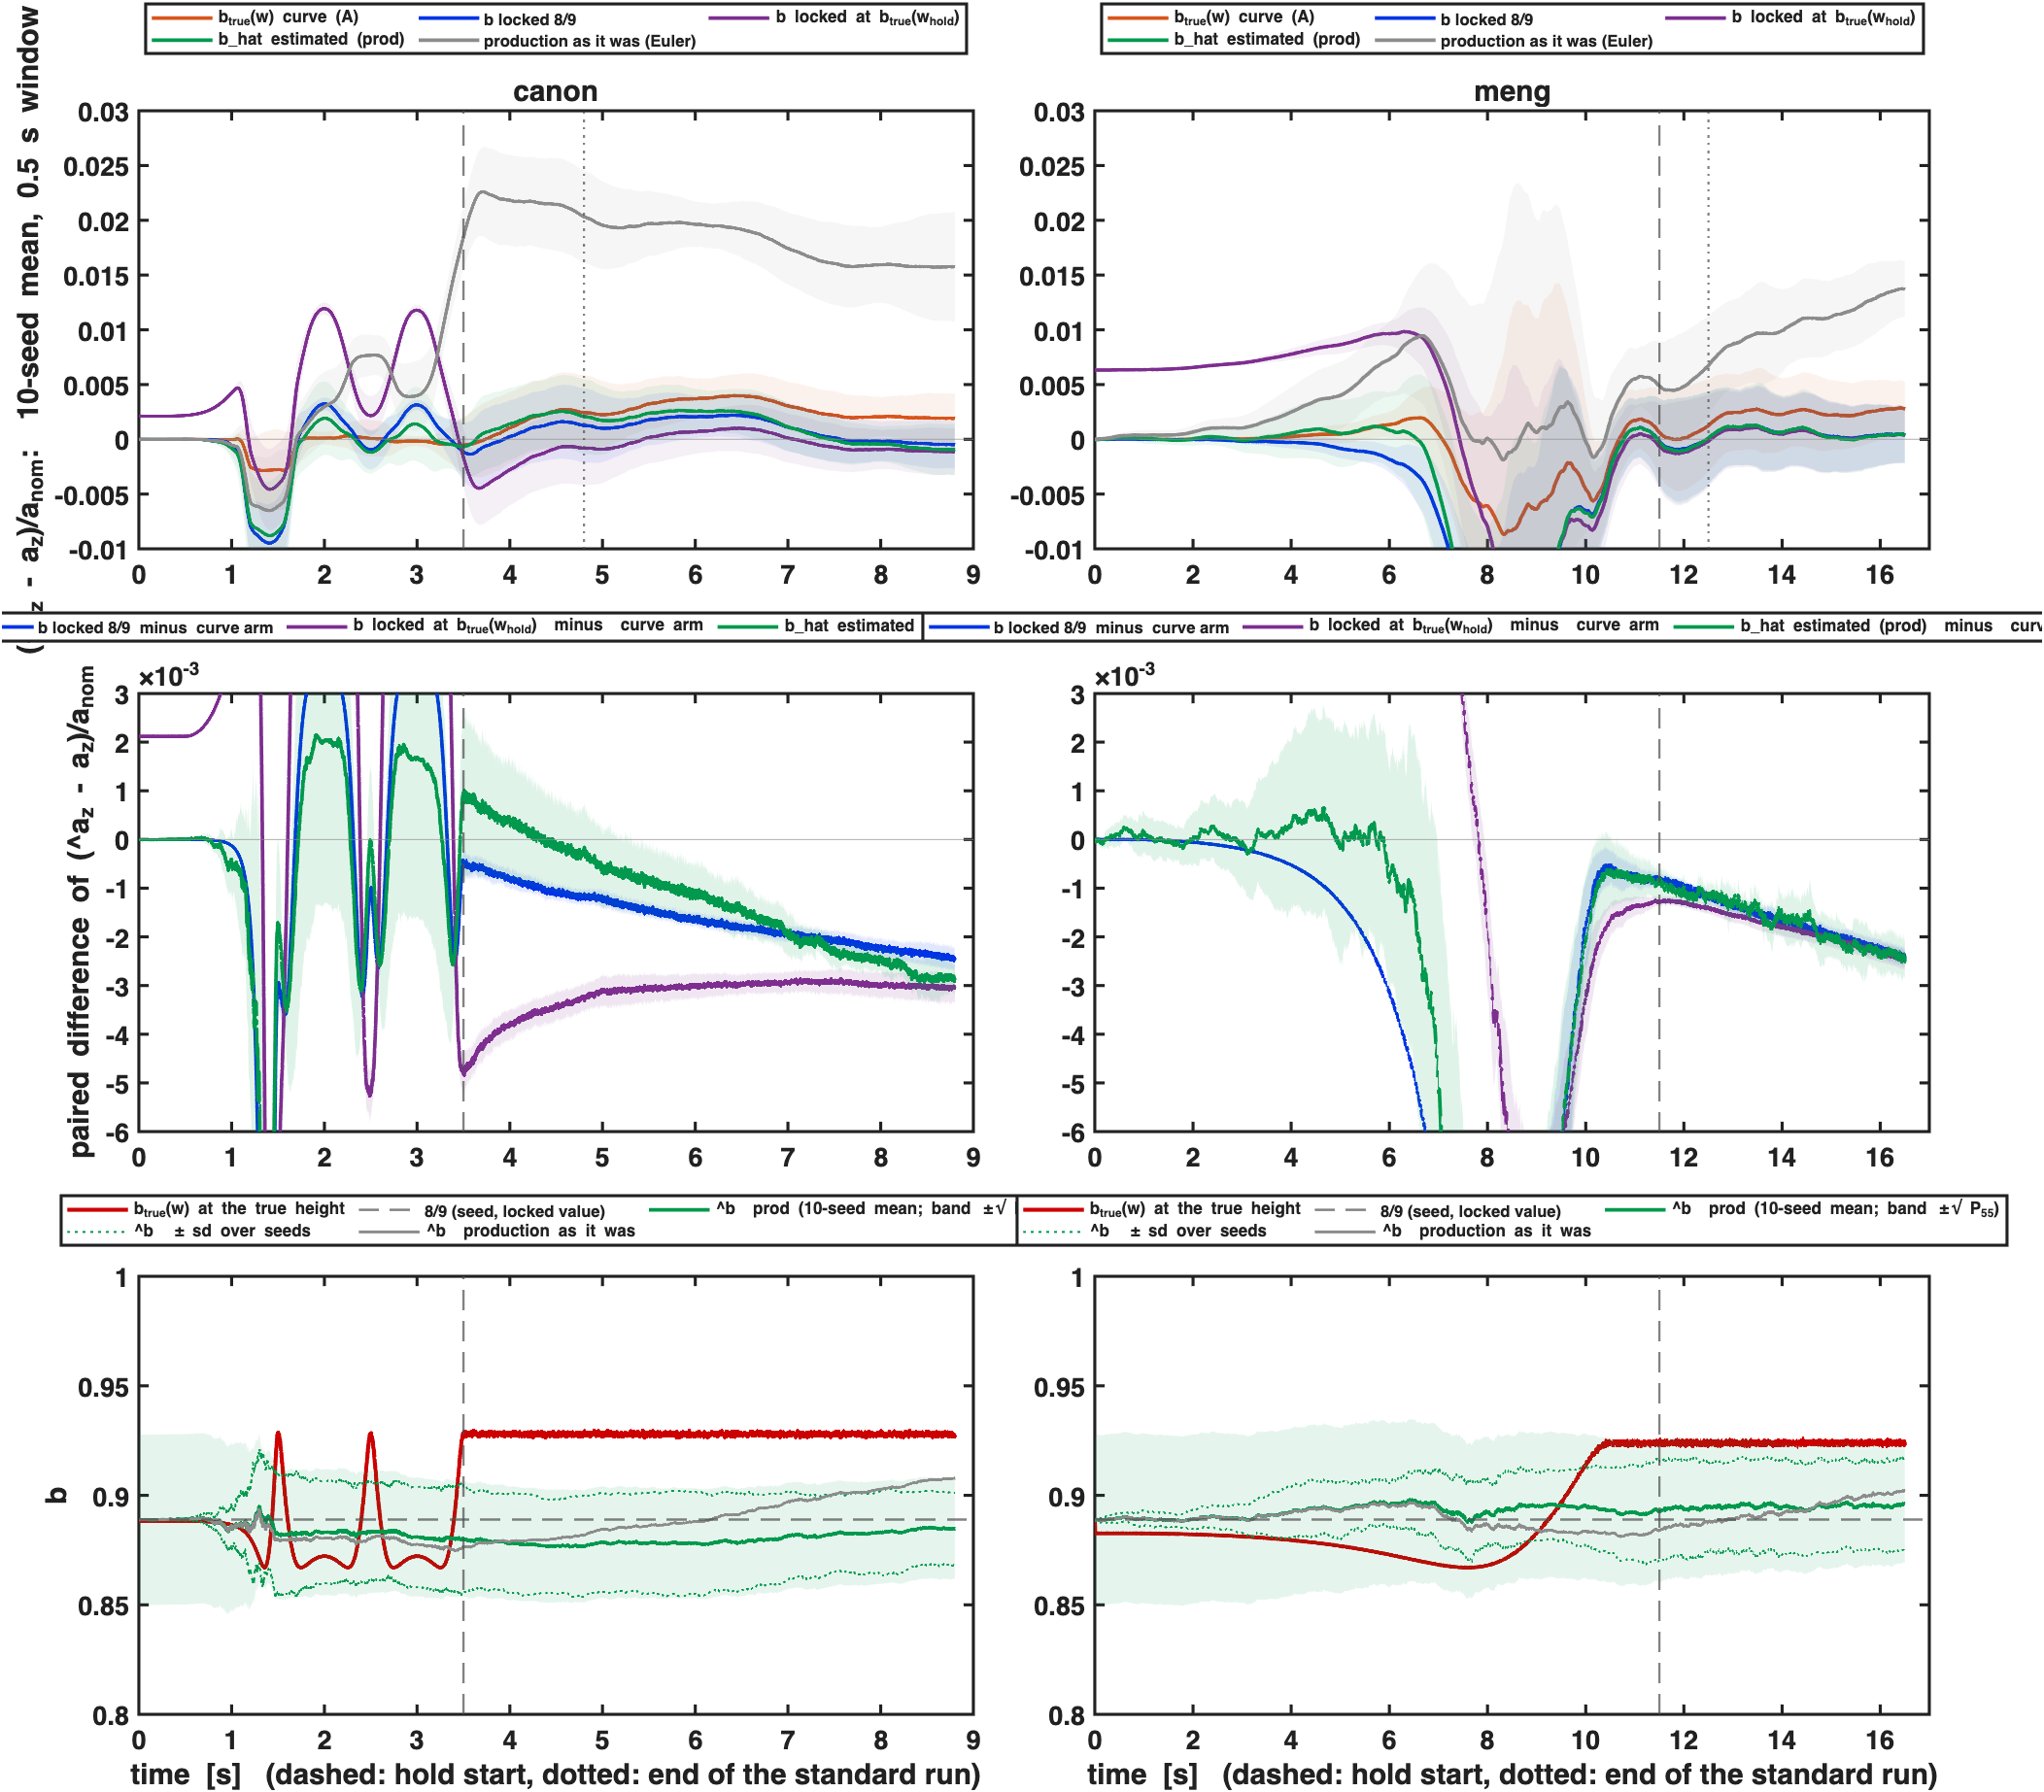
\includegraphics[width=\textwidth]{figures/prod_ladder_band.png}

\clearpage
\thispagestyle{empty}
\noindent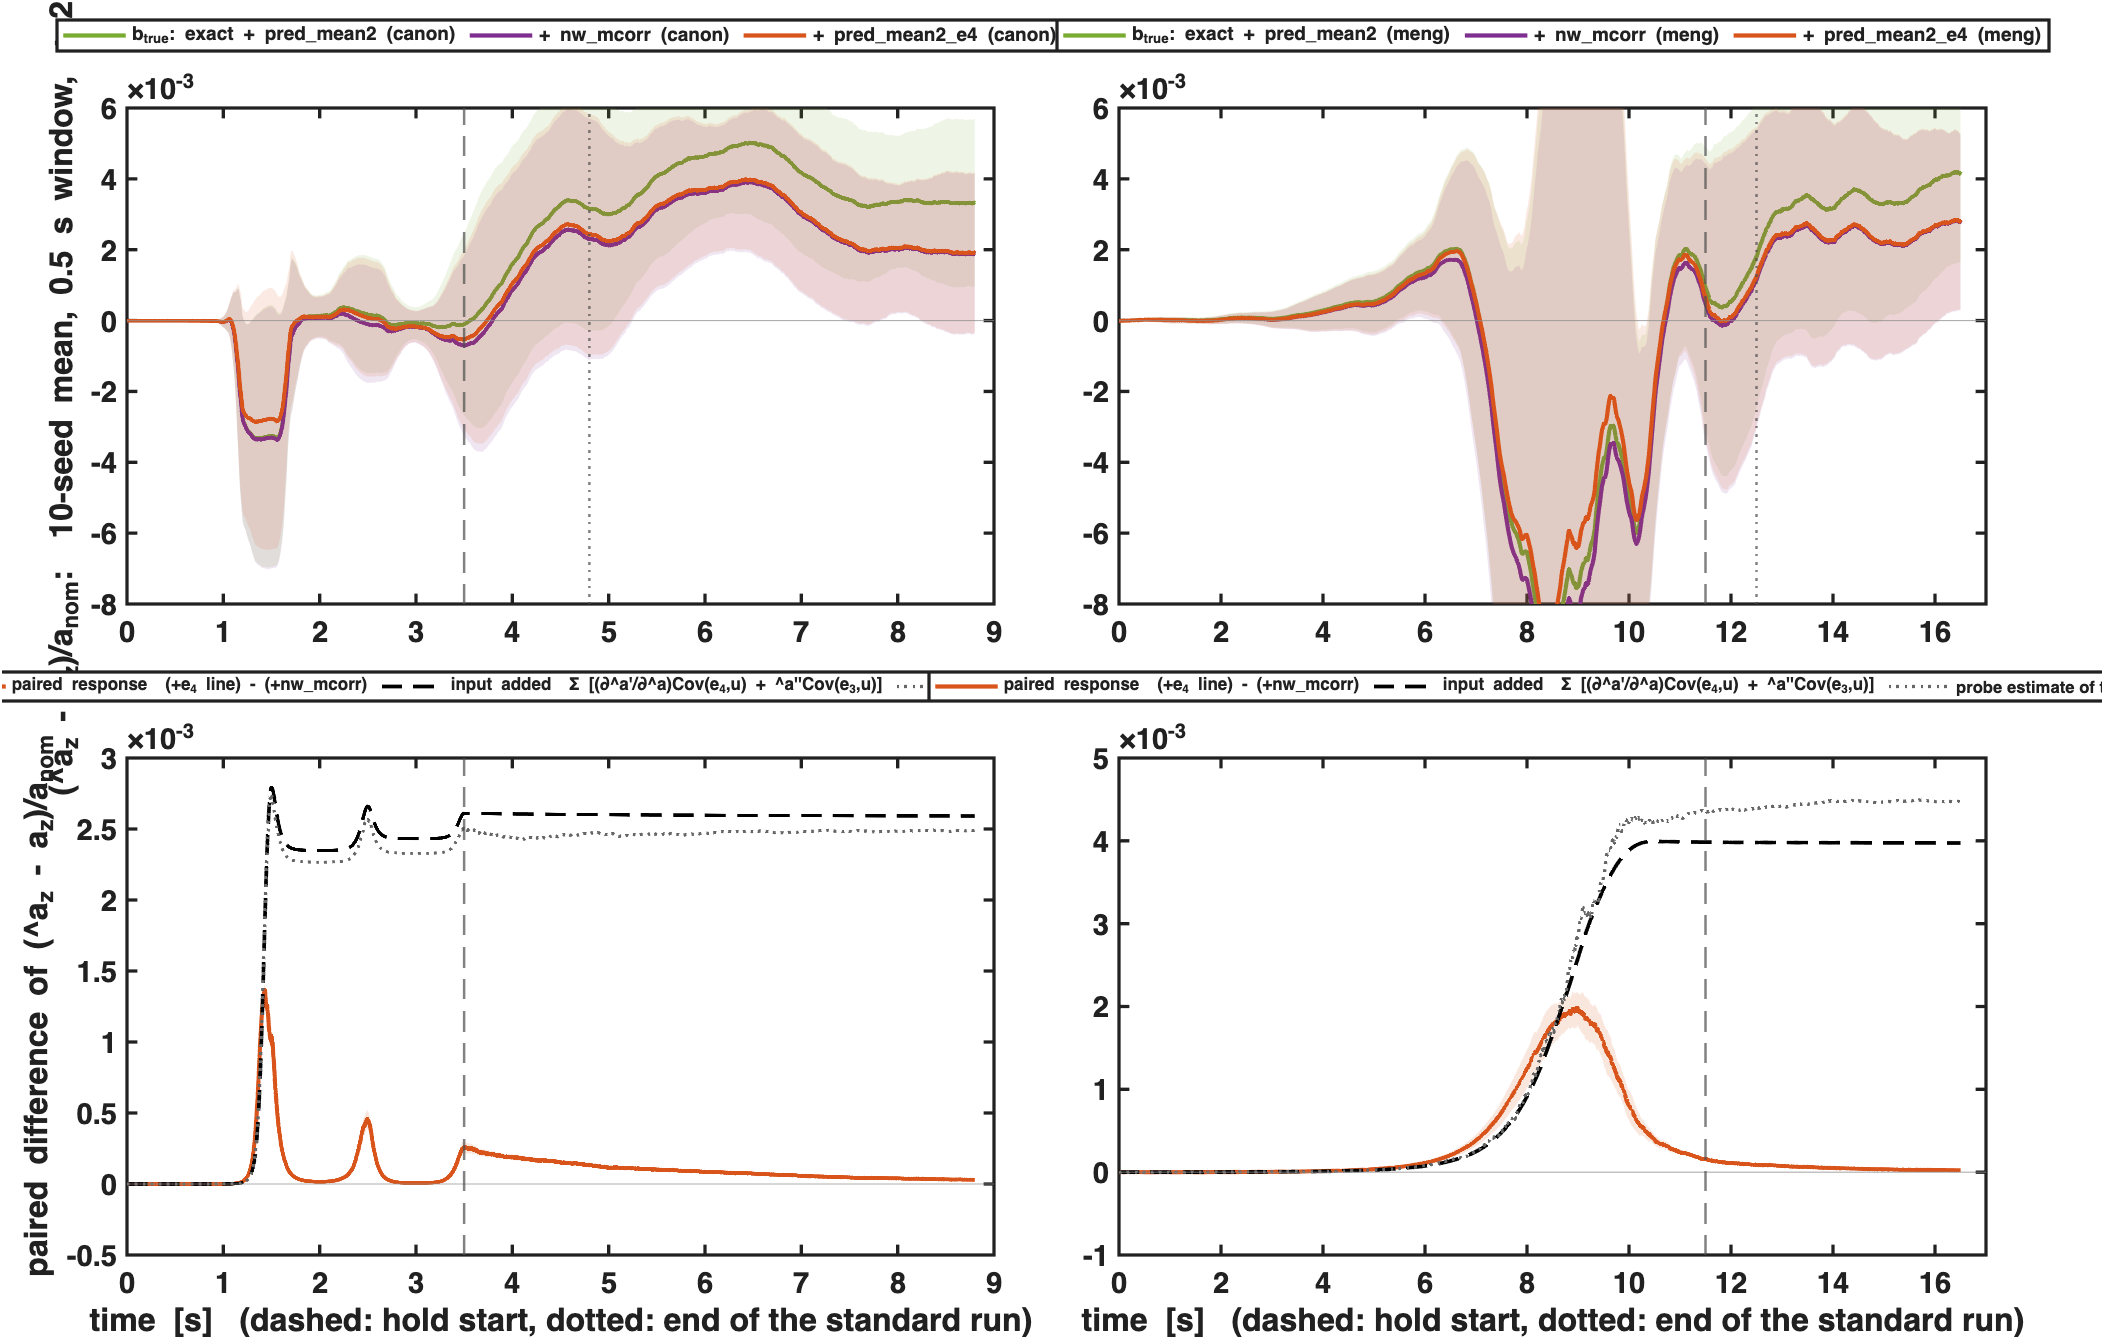
\includegraphics[width=\textwidth]{figures/btrue_three_arms_band.png}

\clearpage
\thispagestyle{empty}
\noindent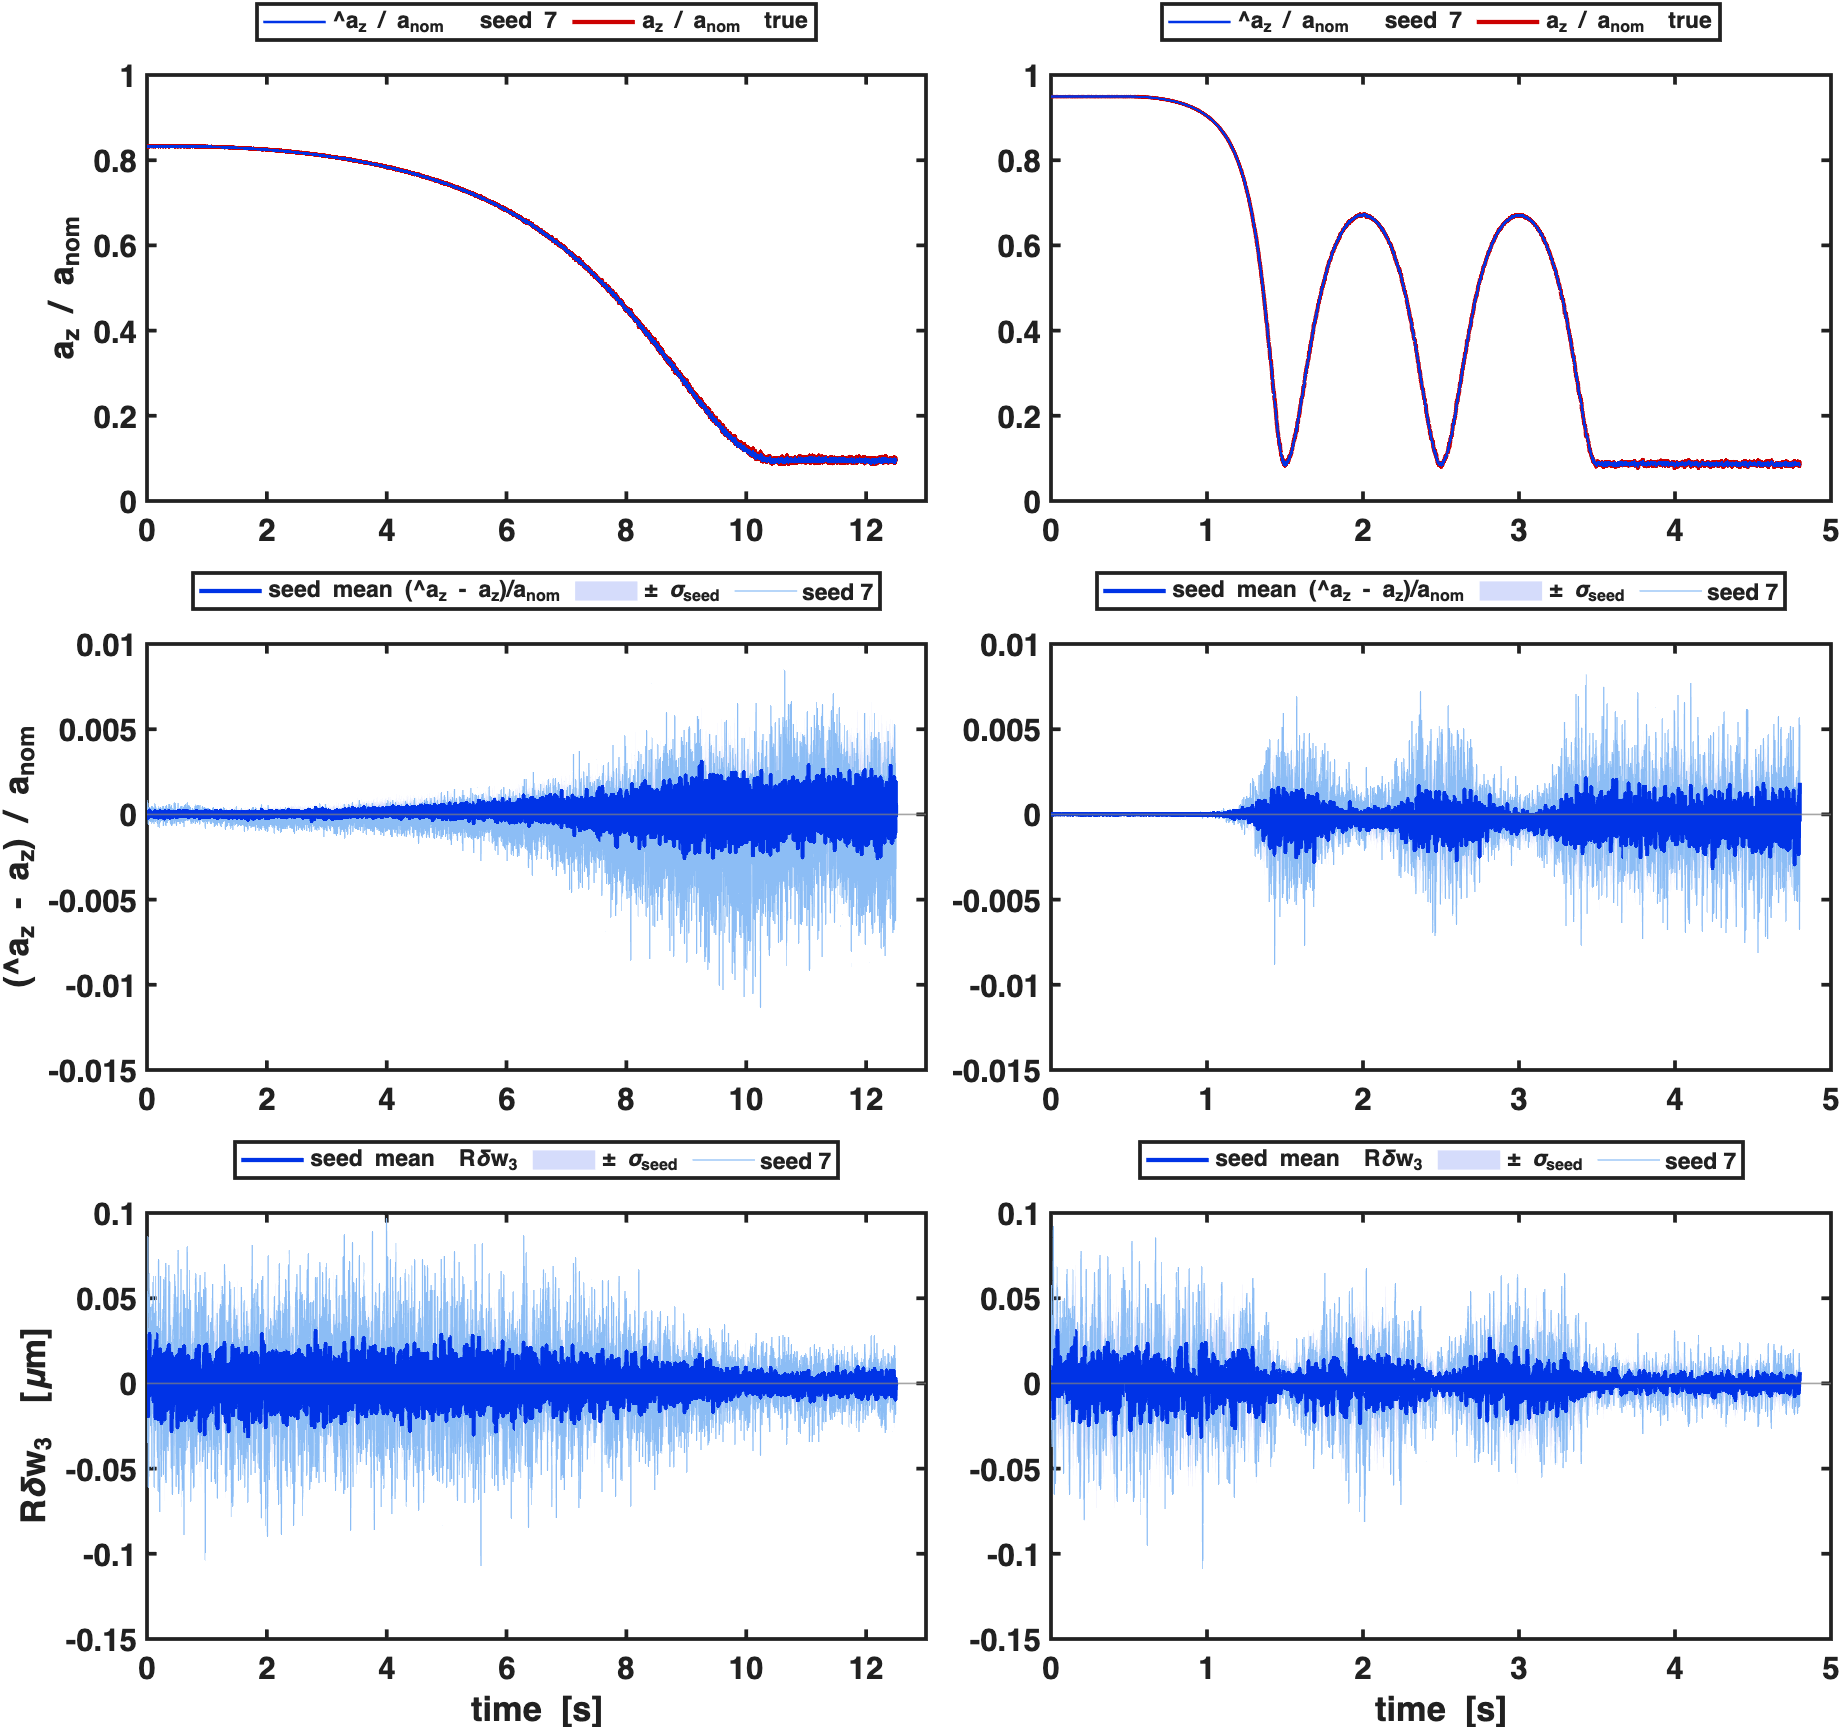
\includegraphics[width=\textwidth]{figures/aptrue_two_traj_final_3row.png}

\end{document}
